% Template for ICIP-2017 paper; to be used with:
% spconf.sty - ICASSP/ICIP LaTeX style file, and
% IEEEbib.bst - IEEE bibliography style file.
% --------------------------------------------------------------------------
%\documentclass[onecolumn]{article}
%\hyphenpenalty=10000\relax
%\exhyphenpenalty=10000\relax
%\sloppy

%\usepackage[preprint]{spconf}
% \copyrightnotice{\copyright\ IEEE 2019}\toappear{\small To appear in {\it Proc.\ IEEE International Conference on Image Processing (ICIP), 2019.}}

\documentclass{article}
\usepackage{spconf}
\usepackage{amsmath,amsfonts,bm,subfig, url}
%\usepackage{spconf,amsmath,bm,subfig}
\usepackage[pdftex]{graphicx}
%\usepackage[dvipdfmx]{graphicx}

\setlength{\abovedisplayskip}{0pt}
\setlength{\belowdisplayskip}{0pt}
% Example definitions.
% --------------------
\def\x{{\bm x}}
\def\y{{\bm y}}
\def\L{{\cal L}}
\newcommand{\argmin}{\mathop{\mathrm{arg~min}}\limits}
% Title.
% ------
%\title{SVD for Constant-time Bilateral Filtering}
\title{200 FPS Constant-time Bilateral Filter Using SVD and Tiling Strategy}
%
% Single address.
% ---------------

\name{Kenjiro Sugimoto$^\dagger\sthanks{This work was supported by JSPS KAKENHI JP17H01764, 18K18076.}$, Norishige Fukushima$^\ddagger$\sthanks{This work was supported by JSPS KAKENHI JP17H01764, 18K19813.}, and Sei-ichiro Kamata$^\dagger$}
\address{$^\dagger$Waseda University, Japan\\
$^\ddagger$Nagoya Institute of Technology, Japan}

%
% For example:
% ------------
%\address{School\\
% Department\\
% Address}
%
% Two addresses (uncomment and modify for two-address case).
% ----------------------------------------------------------
%\twoauthors
% {A. Author-one, B. Author-two\sthanks{Thanks to XYZ agency for funding.}}
% {School A-B\\
% Department A-B\\
% Address A-B}
% {C. Author-three, D. Author-four\sthanks{The fourth author performed the work
% while at ...}}
% {School C-D\\
% Department C-D\\
% Address C-D}
%
\begin{document}
%\ninept
%
\maketitle
%
\begin{abstract}
%100-150 words
This paper presents a constant-time bilateral filter that supports arbitrary range kernel designed via singular value decomposition (SVD). 
Bilateral filter (BF) suffers from high computational complexity in real-time processing due to the time-variant kernel.
Although various accelerations for BF have been proposed, most of them have not achieved both arbitrary range kernel and tight computational complexity simultaneously.
The proposed method supports arbitrary range kernel but requires half computational complexity of most state-of-the-art methods.
Moreover, we present two implementation techniques well matched to the SVD approach: range fitting and tiling strategy.
Experiments show that, in the cases of major range kernels, the proposed method not only runs faster (200 FPS) but also achieves higher accuracy than the state-of-the-art methods.
\end{abstract}
%
\begin{keywords}
SVD, constant-time bilateral filtering, edge-preserving filtering, acceleration
\end{keywords}
%
\section{Introduction}
\label{s.introduction}
Bilateral filter (BF)~\cite{tomasi1998bilateral,elad2002origin} is one of the major edge-preserving smoothing methods widely used in image processing.
Various applications have utilized BF such as denoising~\cite{zhang2008multiresolution}, high dynamic range imaging~\cite{durand2002fast}, detail enhancement~\cite{farbman2008edge}, deblurring~\cite{dai2007bilateral,cho2009fast}, stereo matching~\cite{matsuo2015efficient}, haze removing~\cite{fukushima2018guided}, depth map refinement~\cite{matsuo2013weighted}, optical flow estimation~\cite{fujita2015cost} and so on.
BF smoothes an image using a composite kernel depending on pixel position (spatial kernel) and pixel intensity (range kernel).
Because the kernel shape differs for each target pixel, the computational complexity is much higher than linear filters such as Gaussian filter (GF).

In order to overcome this difficulty, many accelerated algorithms have been proposed in the past. Most of them share the general framework that approximate BF by an appropriate combination of linear filters. The piece-wise linear approximation~\cite{durand2002fast}, an early approach for acceleration, decomposes BF into multiple of GFs implemented by FFT.
Separable BF~\cite{pham2005separable} makes the composite kernel separable to achieve the computational complexity $O(r)$ where $r$ is filter window radius. Unfortunately, this approach causes low accuracy because the composite kernel is essentially nonseparable.
This approach was improved in accuracy in \cite{fukushima2015icassp}.
Another approach for acceleration is a combination with spatial downsampling~\cite{paris2006fast,chen2007real}.
As a more algorithmic improvement, constant-time, or $O(1)$, BF is considered as state-of-the-art for this topic where constant-time means the per-pixel complexity does not depend on filter window radius $r$.
The first method~\cite{porikli2008constant} utilized integral histogram~\cite{porikli2005integral}.
Real-time $O(1)$ BF~\cite{yang2009realtime} further accelerates it using recursive GF~\cite{derich1992recursively,deriche1993recursively}.
The raised cosine based approximation~\cite{chaudhury2011constant,chaudhury2011fast,chaudhury2013acceleration}, compressive bilateral filtering~\cite{sugimoto2015compressive,deng2017fast}, Taylor decomposition based approximation~\cite{chaudhury2015fast,chaudhury2016fast}, and eigenvalue decomposition (EVD) based approach~\cite{sugimoto2016consant} well approximate BF than the piece-wise linear approximation.

Recently, a remarkable technique has been reported for reducing the computational complexity. 
Deng~\cite{deng2017fast} succeeded to reduce the number of GFs by half as compared with \cite{sugimoto2015compressive} by sharing the results of GFs for the numerator and denominator of BF.
However, the range kernel is limited to Gaussian.
Although the EVD method \cite{sugimoto2016consant} supports arbitrary range kernel, the combination with convolution sharing has not been found yet.
The polynomial approximations~\cite{chaudhury2015fast,chaudhury2016fast} shares numerator/denominator convolutions but are limited to differentiable range kernel.
Table~\ref{t:review} lists characteristics of each method.

\begin{table}[tb]
\centering
\caption{Characteristics of major accelerated BFs.}
\vspace{-3mm}
\label{t:review}
\small{
\begin{tabular}{l|c|c}
               & Kernel type        & Conv. sharing     \\ \hline\hline
Linear~\cite{yang2009realtime}         & \textbf{Arbitrary} & N/A               \\ \hline
Raised Cosine~\cite{chaudhury2011constant,chaudhury2011fast,chaudhury2013acceleration}   & Gaussian            & N/A               \\ \hline
Polynomial~\cite{chaudhury2015fast,chaudhury2016fast}         & Differentiable     & \textbf{Possible} \\ \hline
Compressive BF~\cite{sugimoto2015compressive,deng2017fast}    & Gaussian            & \textbf{Possible} \\ \hline
EVD~\cite{sugimoto2016consant,papari2017fast}            & \textbf{Arbitrary} & N/A               \\ \hline
SVD (Proposed) & \textbf{Arbitrary} & \textbf{Possible}
\end{tabular}
}
\vspace{-5mm}
\end{table}

This paper presents an accelerated $O(1)$ BF for the arbitrary range kernel that provides convolution sharing.
We overcome the difficulty using singular value decomposition (SVD).
Our contributions are as follows:
1) Our SVD method reduces the number of convolutions by half by sharing the results of GFs in the numerator and denominator of BF,
2) Our method supports arbitrary range kernels,
and 3) Our method enhances both computational complexity and approximate accuracy by using image tiling strategy and range fitting.
%The proposed method worked within 5 ms for 1 MPixel ($1024 \times 1024$) images on only standard CPU (without GPU computation).


\section{$O(1)$ bilateral filtering}

Let us discuss a $D$-dimensional $R$-tone grayscale image $f:\mathcal{S}\mapsto\mathcal{R}$ where $\mathcal{S}\subset\mathbb{Z}^D$ denotes the domain of pixel positions and $\mathcal{R}=\{0,\ldots,R-1\}\subset\mathbb{Z}$ denotes dynamic range (generally, $D=2$ and $R=256$). Using a pixel position $\bm{p}\in\mathcal{S}$ and its intensity $f_{\bm{p}}\in\mathcal{R}$, BF~\cite{tomasi1998bilateral} is defined by
\vspace{-1mm}
\begin{align}
    \hat{f}_{\bm{p}} &= \frac{
        \sum_{\bm{q}\in\mathcal{S}} w_s(\bm{p},\bm{q})w_r(f_{\bm{p}},f_{\bm{q}})f_{\bm{q}}
    }{
        \sum_{\bm{q}\in\mathcal{S}} w_s(\bm{p},\bm{q})w_r(f_{\bm{p}},f_{\bm{q}})
    }, \label{eq:bilateral}
\end{align}
where $w_s:\mathcal{S}\times\mathcal{S}\mapsto\mathbb{R}$ is spatial kernel and $w_r:\mathcal{R}\times\mathcal{R}\mapsto\mathbb{R}$ is range kernel.
The most common choice is Gaussian:
\vspace{-1mm}
\begin{align}
    w_s(\bm{p},\bm{q}) &= e^{-\frac{\| \bm{q}-\bm{p} \|_2^2}{2\sigma_s^2}}, &
    w_r(a,b) &= e^{-\frac{\left( b-a \right)^2}{2\sigma_r^2}}
\label{eq:kernels}
\end{align}
where $\sigma_s\in\mathbb{R}_+$ is spatial scale and $\sigma_r\in\mathbb{R}_+$ is range scale.

In $O(1)$ BF~\cite{sugimoto2015compressive,deng2017fast,sugimoto2016consant,papari2017fast}, the range kernel is generally approximated by separable form $w_r(a,b) \approx \sum_{k=0}^{K-1} \phi_k(a) \psi_k(b)$. By plugging it to \eqref{eq:bilateral},
\vspace{-1mm}
\begin{align}
    \hat{f}_{\bm{p}}\!&\approx\!\frac{
        \sum_{k=0}^{K-1} \phi_k(f_{\bm{p}})
        \sum_{\bm{q}\in\mathcal{S}} w_s(\bm{p},\bm{q}) \{ \psi_k(f_{\bm{q}}) f_{\bm{q}} \}
    }{
        \sum_{k=0}^{K-1} \phi_k(f_{\bm{p}}) 
        \sum_{\bm{q}\in\mathcal{S}} w_s(\bm{p},\bm{q}) \{ \psi_k(f_{\bm{q}}) \}
    }.
\label{eq:bilateral-o1}
\end{align}
In this equation, $\{\cdot\}$ can be regarded as intermediate images and $\sum_{\bm{q}\in\mathcal{S}}$ indicates their convolution.
This separable approximation results in BF decomposed into a product sum of $2K$ convolutions.
By implementing the convolutions as $O(1)$ filters including~\cite{sugimoto2013fast,sugimoto2015efficient,sugimoto2018universal},
BF~\eqref{eq:bilateral-o1} can run in $O(1)$ time per pixel.
In this framework, our purpose is to achieve higher approximate accuracy using the smaller number of convolutions, or intermediate images.
In existing methods, as $\phi_k(\cdot)$ and $\psi_k(\cdot)$ in ~\eqref{eq:bilateral-o1}, trigonometric functions~\cite{sugimoto2015compressive,deng2017fast} for the Gaussian range kernel, and eigenvectors for arbitrary kernels~\cite{sugimoto2016consant,papari2017fast} have been used.

As a remarkable approach, \cite{deng2017fast} succeeded to reduce the number of convolutions by half by sharing the results of convolutions in the numerator and denominator of \eqref{eq:bilateral-o1}. However, this method does not ensure to minimize least-squares error.

%\vspace{-4mm}
\section{Proposed Method}
%\vspace{-3mm}
\subsection{Range Kernel Decomposition via SVD}

We propose $O(1)$ BF that supports convolution sharing for arbitrary range kernel approximated in the least-squares manner.
Inspired from \cite{deng2017fast}, we reformulate \eqref{eq:bilateral} as
\vspace{-1mm}
\begin{align}
    \hat{f}_{\bm{p}}-f_{\bm{p}} &= \frac{
        \sum_{\bm{q}\in\mathcal{S}} w_s(\bm{p},\bm{q})w_r(f_{\bm{p}},f_{\bm{q}})(f_{\bm{q}}-f_{\bm{p}})
    }{
        \sum_{\bm{q}\in\mathcal{S}} w_s(\bm{p},\bm{q})w_r(f_{\bm{p}},f_{\bm{q}})
    }.
\label{eq:bilateral-diff}
\end{align}
By newly defining $\tilde{w}_r(a,b)=w_r(a,b)(b-a)$, we also decompose it into $\tilde{w}_r(a,b) \approx \sum_{k=0}^{K-1} \tilde{\phi}_k(a) \tilde{\psi}_k(b)$ in the numerator.
Substituting them for~\eqref{eq:bilateral-diff}, BF is rewritten as
\vspace{-1mm}
\begin{align}
    \hat{f}_{\bm{p}}\!-\!f_{\bm{p}} &\approx \frac{
        \sum_{k=0}^{K-1} \tilde{\phi}_k(f_{\bm{p}})
        \sum_{\bm{q}\in\mathcal{S}} w_s(\bm{p},\bm{q}) \{ \tilde{\psi}_k(f_{\bm{q}}) \}
    }{
        \sum_{k=0}^{K-1} \phi_k(f_{\bm{p}})
        \sum_{\bm{q}\in\mathcal{S}} w_s(\bm{p},\bm{q}) \{ \psi_k(f_{\bm{q}}) \}
    }.
\label{eq:bilateral-ours}
\end{align}
If $\psi_k(a,b)=\tilde{\psi}_k(a,b)$, we can share the convolution results of the numerator and denominator, which means the number of the convolutions is reduced from $2K$ to $K$.

We can find such a kernel decomposition via SVD.
First, we introduce $\bm{W},\tilde{\bm{W}}\in\mathbb{R}^{R \times R}$ and $\bm{W}[a,b]=w_r(a,b)$, $\tilde{\bm{W}}[a,b]=\tilde{w}_r(a,b)$ where $[\cdot]$ denotes element accessing operator. By applying SVD to the vertically-connected matrix $\bm{X}=[\bm{W}^\top,\tilde{\bm{W}}^\top]^\top\in\mathbb{R}^{2R \times R}$,
they can be approximated by the top-$K$ components.
Using the singular vectors, each element of $\bm{X}$ can be represented as the separable form
\vspace{-1mm}
\begin{align}
    \bm{X}[a,b] &\approx \sum_{k=0}^{K-1} \sigma_k \bm{u}_k[a] \bm{v}_k^\top[b],
\label{eq:tsvd}
\end{align}
where $\sigma_k$ ($\sigma_0\geq\ldots\geq\sigma_{K-1}$) is the $k$-th singular value,
and $\bm{u}_k\in\mathbb{R}^{2R}$, $\bm{v}_k\in\mathbb{R}^{R}$ are the left/right singular vectors.
If we set to $\psi_k(b)=\tilde{\psi}_k(b)=\sigma_k \bm{v}_k[b]$, the intermediate images are shared. Similary, we obtain $\phi_k(a)=\bm{u}_k[a]$ and $\tilde{\phi}_k(a)=\bm{u}_k[a+R]$.
Thus, we can perform \eqref{eq:bilateral-ours} by $K$ convolutions.

%\vspace{-4mm}
\subsection{Range Fitting}
%\vspace{-0.5mm}

\begin{figure}[t]
\centering
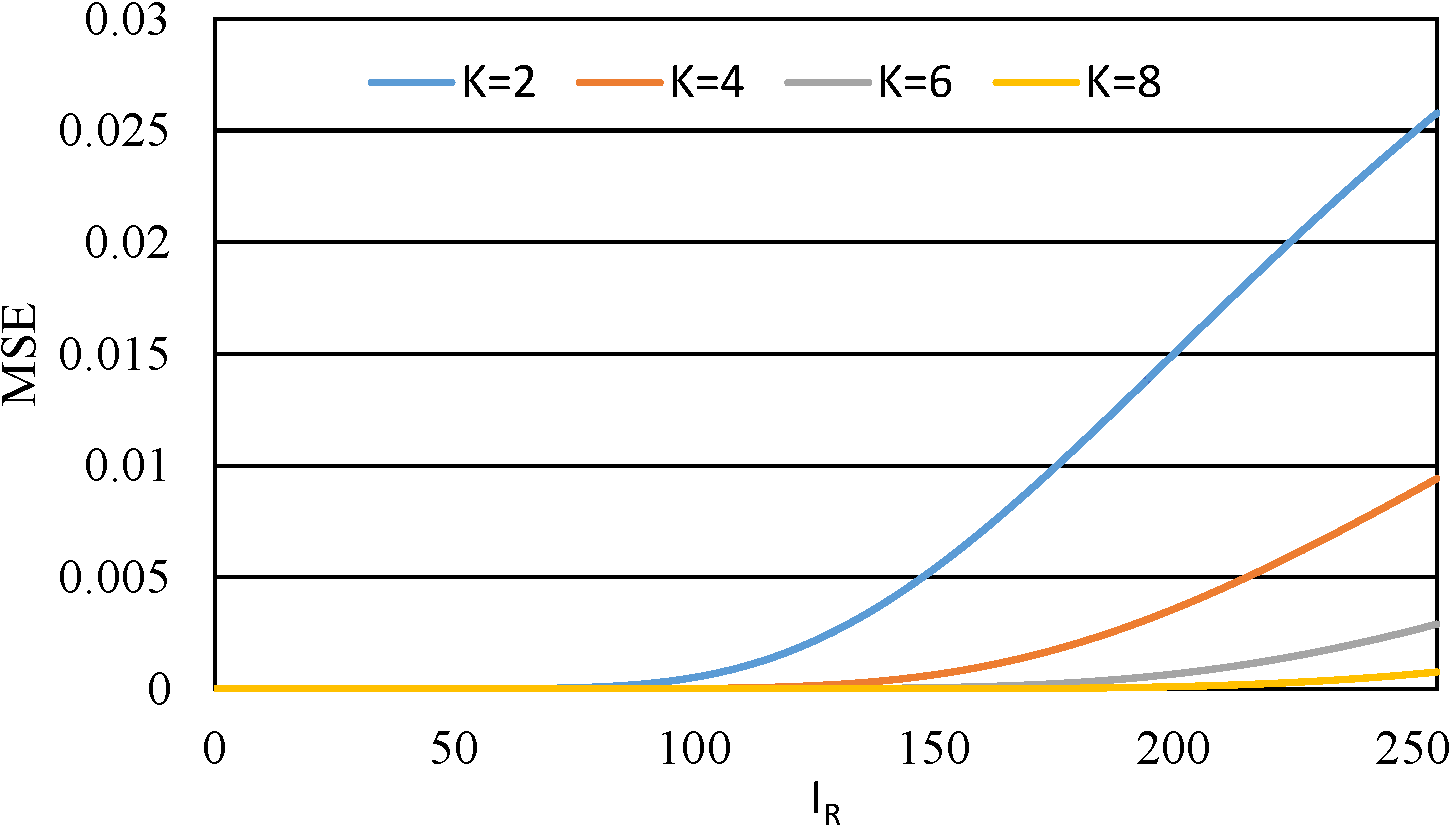
\includegraphics[width=0.7\columnwidth]{fig/error_EVD_MSE.pdf}
\vspace{-2mm}
\caption{MSE of kernel approximation via SVD.}
%\vspace{-4mm}
\label{f:svdmse}
\end{figure}

The default dynamic range in an image is usually $[0:255]$, but the actual range depends on the image content.
We do not use out of the actual range in the bilateral filter; thus, we can reduce the matrix size of $\bm{W}$ by $I_{\min}$ and $I_{\max}$, where the minimum and maximal intensity in the input image.
We call the process, \textit{range fitting}.
After the range fitting, the least square error in the approximated range kernel becomes small.
Based on the Frobenius norm, the mean least square error between the ideal range kernel and the approximated one is defined as:
\vspace{-1mm}
{
\small
\begin{align}
e(K,\!I_{R}) \!=\!\! \frac{\sum_{a=I_{\min}}^{I_{\max}}\!\sum_{b=I_{\min}}^{I_{\max}}\{ w_{r}(a,\!b) \!-\! \sum _{k=0}^{K-1} \sigma_{k} \bm{u}_{k}[a]\bm{v}_{k}[b]) \}^2}{(I_{R}+1)\times (I_{R}+1)}.
\end{align}
}
Figure~\ref{f:svdmse} shows the error for with respect to $I_R = I_{\max}-I_{\min}$ and $K$.
When $I_R$ is small, the error of the kernel is small; thus, we approximate the bilateral filtering well.
The performance of the range filtering is further improved by tiling, which is introduced in the next section.

The SVD computation is overhead costs; thus, we utilize look-up tables (LUTs) to save the computational time.
For computing the range kernel based on the SVD, we need the $k$-th singular value vectors $\bm{u}_k$ and matrix multiplying results of the singular value vectors and the matrix $\bm{W}$.
To keep the resulting values, the size of the LUT is $K \times I_R$.
The value is changed based on $\sigma_r$, $K$, and $I_R$.
Therefore, we should pre-compute the values for each parameter for the LUT.
%なおこのほかにもSVDの効率化のためにいくつかのアイデアを導入しているが紙面の都合でその説明は割愛する.

%主要な計算はSVDであるため,もし行列積をプレプロセスで行うのであれば,サイズnxTだけLUTからロードすればよい.
%ただし,今回は,3つともLUTからロードした.

\subsection{Efficient Computational Scheduling}

This section discusses efficient computational scheduling of $O(1)$ BF.
In general, the whole process of \eqref{eq:bilateral-ours} consists of four subprocesses: decomposition $D$, convolution $C$, product sum $P$ and normalization $N$.
After precomputation such as SVD, we first generate some intermediate images from an input image as
\begin{align}
    D(\bm{p},k) &= \psi_k(f_{\bm{p}}) = \tilde{\psi}_k(f_{\bm{p}}).
\end{align}
All the intermediate images are then convolved with spatial kernel $w_s$ as
\begin{align}
    C(\bm{p},k) &= \sum_{\bm{q}\in\mathcal{S}} w_s(\bm{p},\bm{q}) D(\bm{p},k)
\end{align}
If it is Gaussian spatial kernel, one can use an efficient $O(1)$ GF such as ~\cite{sugimoto2013fast,sugimoto2015efficient,sugimoto2018universal} instead of na\"ive Gaussian convolution, which results in $O(1)$ BF.
After computing two product-sums from these results, we normalize the results for each pixel as
\begin{align}
    N(\bm{p}) &= \frac{P_\mathrm{N}(\bm{p})}{P_\mathrm{D}(\bm{p})}
        = \frac {\sum_{k=0}^{K-1} \tilde{\phi}_k(f_{\bm{p}})~C(\bm{p},k)}
                {\sum_{k=0}^{K-1} \phi_k(f_{\bm{p}})~C(\bm{p},k)}.
\end{align}
Note that the intermediate image $C(\bm{p},k)$ is shared both in numerator and denominator. These subprocesses should be efficiently operated in real-time processing.

We design the whole process by utilizing parallel processing on the CPU.
Here, we assume 2D image filtering, i.e., $\bm{p}=[x,y]^\top$.
In most cases, it is adequate to parallelize the outermost loop for efficient parallel computation.
Since the $D$, $C$, and $P$ steps contain triple loops ($x, y, k$) and the $N$ step has double loops ($x,y$), parallelizing the $k$-loop seems the most effective.
The important point is that the number of elements must be sufficiently more massive than the number of CPU cores for parallelizing load balance.
Since the number of $k$ is 4--20 in general, parallelizing the second outer loop with respect to $y$ could be effective.

The $C$ step is an exception because we use recursive processing for effective convolution~\cite{sugimoto2013fast,sugimoto2015efficient,sugimoto2018universal}.
The recursive filter has a dependency on the processing pixel order of $x$ and $y$.
In this case, we should parallelize the $k$-loop.
Considering memory cache and processing pipeline, parallelizing the $k$-loop in the step before convolution seems better depending on the processing unit.
In the remaining loops, $y$ loop parallelization is effective.
As described in computing steps, the $O(1)$ BF has multiple \textit{fork-join} parallel processes and the complex image processing pipeline.
Therefore, it has low parallelization efficiency and low cache efficiency.

We overcome this difficulty by image tiling strategy, which is a major loop optimization technique for compilers.
Tiling strategy enables the $x$ and $y$ loops to be split to contain loaded data in processing unit cache to improve cache efficiency.
Besides, by processing each tile in parallel, the parallel ability is also improved.
Note that, as the blue region in Fig.~\ref{f:tile} shows, it is required for supporting parallel processing to care about additional $2r$ pixels for each tile in the convolution step.

%加えて,分解,畳み込み,内積の処理をインタリーブして行うことで,必要なバッファサイズを大きく削減可能である.
%(分母画像,分子画像,中間バッファ画像の画像3枚分である.一方で,インタリーブしない場合は,これの次数n倍のメモリを消費する.)
%このようにすると計算効率が大きく向上する.
\begin{figure}[t]
\centering
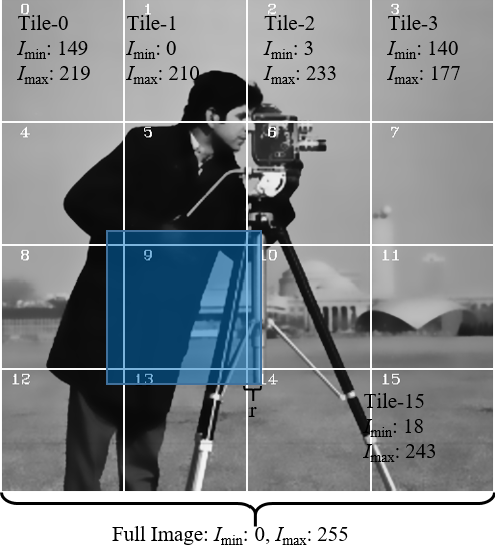
\includegraphics[width=0.6\columnwidth]{fig/tile.pdf}
\caption{Illustration of $4 \times 4$ tiling. The subimages are expected to have lower contrast (narrower range) than the full image.}
\label{f:tile}
\end{figure}

More importantly, the tiling strategy improves the performance of range fitting.
As Fig.~\ref{f:tile} indicates, each subimage tends to represent local texture such as flat or edge parts.
In natural images, a local region shows lower contrast, i.e., narrow intensity range.
Specifically, $I_{R}=I_{\max}-I_{\min}$ for each subimage is expected to be smaller than the full image.
This mechanism is matched to our SVD approach: narrower range contributes to lower computation cost.

%We can regard the tiling-processing that multi-core processors simultaneously filter a number of small images.

\section{Experimental Results}

We evaluated the real performance of our method for approximation accuracy and computational time. 
All the codes were implemented in C++, developed on Visual Studio 2017 parallelized by OpenMP and vectorized by AVX/AVX2. 
Approximate accuracy is quantified as Peak Signal-to-Noise Ratio (PSNR) between the ideal result (original BF) and filter output.

In the first experiment, we justified approximation accuracy and computational performance of BF with Gaussian range kernel. We compared the proposed method with Compressive BF (CBF)~\cite{sugimoto2015compressive}, its acceleration method called Fast Compressive BF (FCBF)~\cite{deng2017fast} and the EVD-based method~\cite{sugimoto2016consant}. Note that CBF and EVD do not share convolutions of numerator/denominator; by contrast, FCBD and SVD (ours) share convolutions of them.
Figure~\ref{f:order_sigma} shows the order of CBF/FCBF and EVD/SVD for the approximation accuracy.
Under the same order, CBF/EVD achieved higher performance than the shared method. When $K$ and $\sigma_r$ are small, which is a hard condition for approximating BF, the shared methods FCBF/SVD outperforms the others.
This is because FCBF/SVD subtract edges from the source image, but EVD/CBF add edges for blurred image.
Resulting images for small $\sigma_r$ are similar to source images in visibility. Hence, the shared methods have superior performance in this condition.
Note that the relation of the order and the number of convolutions is different for each method, such as CBF: $4K+1$, FCBF: $2K$, EVD: $2K$ and SVD: $K$.

In order to consider the actual computational performance, we replot the horizontal axis as computational time.
Figure~\ref{f:time_sigma} plots computational time for the PSNR.
SVD (our method) is faster with almost the same accuracy than FCBF.
Note that all the methods are parallelized and optimized by $4 \times 4$ tiling strategy.

\begin{figure}[t]
\centering
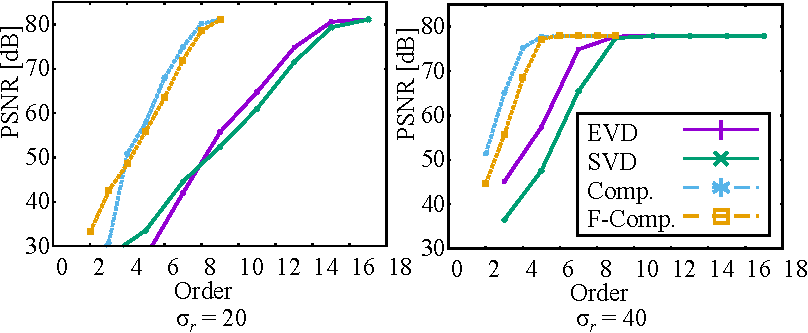
\includegraphics[width=\columnwidth]{fig/order_psnr.pdf}
\vspace{-6mm}
\caption{Order w.r.t. PSNR on various methods ($\sigma_s = 5$).}
\label{f:order_sigma}
\vspace{-3mm}
\end{figure}
\begin{figure}[t]
\centering
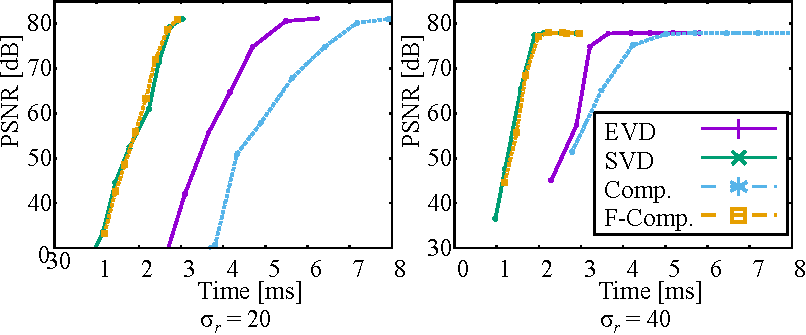
\includegraphics[width=\columnwidth]{fig/time_psnr.pdf}
\vspace{-6mm}
\caption{Computational time [ms] w.r.t. PSNR [dB] on various methods ($\sigma_s = 5$).}
\vspace{-3mm}
\label{f:time_sigma}
\end{figure}

In the second experiment, we confirmed the effectiveness of tiling strategy and range fitting. Figure~\ref{f:scheduling} shows the results of SVD with/without tiling and with/without range fitting. Note that tiling without range fitting (Tiling w/o RF) is the same curve of SVD in Fig.~\ref{f:time_sigma}.
The tiling accelerates $O(1)$ BF significantly.
Range fitting improves the performance for both with/without tiling cases.
Also, the tile-based range fitting further improves performance.
The precomputing overhead for computing $I_{R}$ took only 0.03 [ms].

In the third experiment, we verified that our method was able to approximate various range kernels. We tested hat kernel (or the Bartlett window, triangular window), defined by
%\vspace{-1mm}
\begin{align}
w_r(a,b) := \max(|a-b|,0).
\label{eq:th}
\end{align}
and the double exponential (or Laplace) distribution kernel, defined by
\begin{align}
w_r(a,b) := e^{-\frac{|a-b|}{\sigma}}.
\label{eq:th2}
\end{align}
Note that this is not Laplacian kernel for edge detection.
Both kernels are non-differentiable and, obviously, not Gaussian.
We compared the proposed method with the linear interpolation approach~\cite{yang2009realtime} and EVD, which support arbitrary range kernels.
Figure~\ref{f:hatlap} reveals performance in the cases of the Bartlett window and the Laplace distribution kernel.
The proposed method clearly outperformed both state-of-the-art methods.

%In the fourth experiment, we verified the computational time of the only SVD for range kernel decomposition and LUT acceleration.
%SVDの時間は,2のべき乗だと速い.
%でも,必要な係数はxxxバイトの配列だけなので,事前に計算しておけば,LUTを使えばxx msで終わる.
%行列Yを用意するのに13ms.高速な計算部分は3ms
%おもな計算時間はGEMMなのでここ速くするともうちょっとまし.


\begin{figure}[t]
\centering
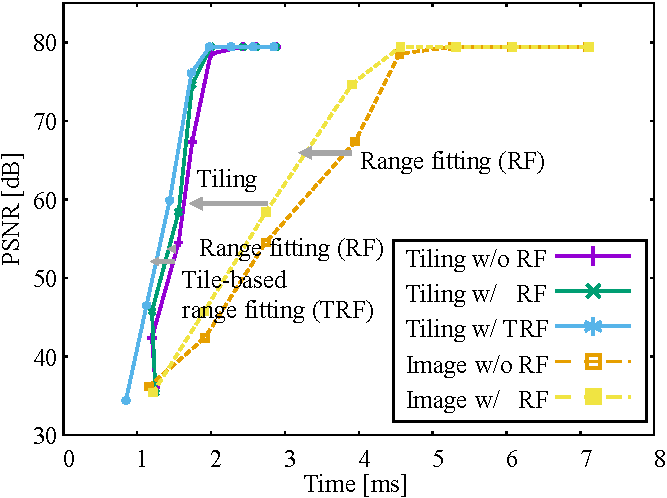
\includegraphics[width=0.8\columnwidth]{fig/schedule.pdf}
\vspace{-4mm}
\caption{SVD of Computational time [ms] w.r.t. PSNR [dB] with/without tiling and with/without range fitting ($\sigma_s = 5$).}
\label{f:scheduling}
\vspace{-3mm}
\end{figure}
\begin{figure}[t]
\centering
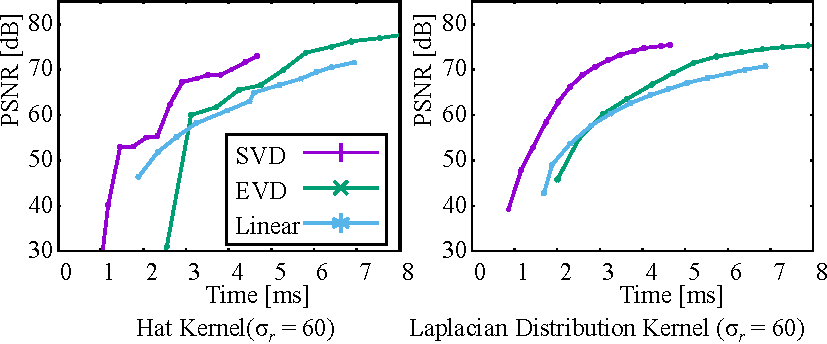
\includegraphics[width=\columnwidth]{fig/hat_lap.pdf}
\vspace{-3mm}
\caption{SVD of Computational time [ms] w.r.t. PSNR [dB] on the hat and Laplacian distribution kernel cases ($\sigma_s = 5$).}
\label{f:hatlap}
\vspace{-2mm}
\end{figure}

\section{Conclusion}

This paper proposed $O(1)$ BF designed via SVD that supports arbitrary range kernel and reduces the number of convolutions by half.
Moreover, image tiling strategy and range fitting improve the performance drastically.
Our method showed higher performance in both accuracy and computational time.
The proposed method achieves sufficient approximation accuracy within 5 ms for arbitrary range kernel approximation in $512\times 512$ size image; thus, the frame rate of our method is over 200 frame per second.
\clearpage
\bibliographystyle{IEEEbib}
\small
\bibliography{icip2019}

\end{document}
